\section{Resultados}
Nesta seção, será debatido acerca dos resultados obtivos por meio dos dois testes realizados. O primeiro visou analisar o tempo médio de cada algoritmo, bem como o desvio padrão. No segundo teste, contudo, buscou avaliar o comportamento dos algoritmos bolha e inserção quando submetidos a listas com a taxa de ordenação. 
%TODO  (colocar aqui as taxas)
Logo abaixo, há o gráfico dos resultados obtidos ao executar cada um dos algoritmos falados e, como complemento, a função do Python.

\begin{figure}[h]
    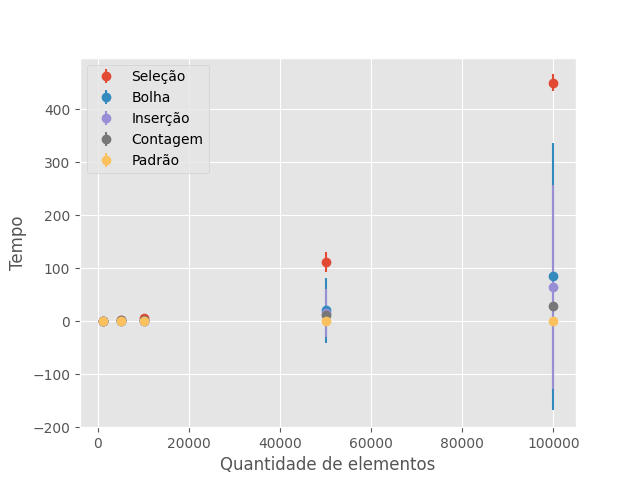
\includegraphics[width=8cm]{sizes.png}
    \caption{Gráfico elucidando o comportamento de cada algoritmo em tópico. No eixo x, há a quantidade de elementos; no y, o tempo médio gasto, em segundos, por cada algoritmo}
    \end{figure}

    \subsection{Ordenação prévia}
    \begin{figure}[h]
        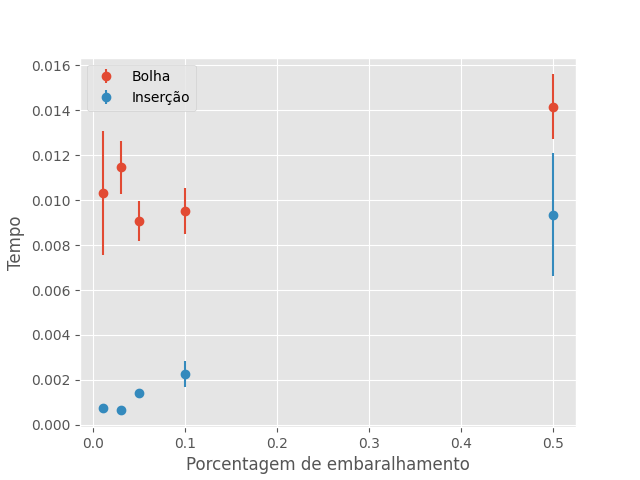
\includegraphics[width=8cm]{result_1717713581.4751563.png}
        \caption{Gráfico ilustrando o tempo médio 'gasto' dos algoritmos bolha e inserção em relação à taxa de ordenação inicial dos vetores.}
    \end{figure}

Como  previamente comentado, o algoritmo de bolha e o de inserção variam de acordo com a taxa de ordenação. Assim, em caso de ordenação inicial total, ambos os algoritmos adquirem um comportamento linear.